\chapter{Project Proposal}
\section{Project Name}
The name for the project is CryptoStats
\section{Overview of the Project}
The aim of the project is to provide users with relevant information regarding cryptocurrency exchanges. By analysing the data provided by the external API on the values of the cryptocurrencys, the service will provide the user with information about the patterns in the value of the cryptocurrency and data such as the average number of days that the currency's value declines and increases in one go, if there is any resemblance in the fluctuation betweeen the currency and other major currencies.

The goal with the project is to be able to provide users with enough information to help them make informed decisions when doing an exchange for a particular coin, and also gather information about what makes cryptocurrenncies fluctuate in value. Rather than just showing the value of the coin, the service aims to provide way more valuable information by analysing the data in the currency's history, which allows the user to posess very important and essential information when trading coins.

The information processed will be presented to the users in two different ways: The first in a web site that will display the data in a user-friendly manner, built using ASP.NET Core 2 for the back-end and Angular and Bootstrap for the front-end. The second is by presenting the processed information to the user through a RESTful API with a JSON response, in order to facilitate the integration of the information with other applications or services.

For the submission of the project, I only intend to provide information for major coins such as Bitcoin, Ethereum, Litecoin and Bitcoin Cash, since they are the most known and there is many information and exchanges that trade these coins.
\section{External Web Services}
In order to obtain information about the coins, I will be using the \href{https://docs.gdax.com}{GDAX exchange API}.


\section{Data Exposed By The Service}
The service aims to expose the following data:
\begin{itemize}
    \item Average fluctuation
    \item Average time when in growth
    \item Average time when in decline
    \item Difference between highest value and latest value
    \item Resemblance in curb with other cryptocurrencies
\end{itemize}
\section{Database Schema}
\begin{center}
    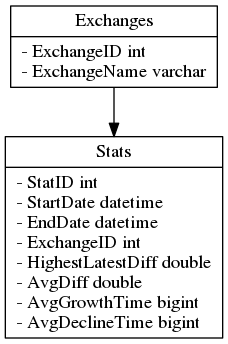
\includegraphics{dbschema.png}
\end{center}


\section{User Interface Ideas}